\documentclass[10pt,letterpaper]{article}

\usepackage[utf8]{inputenc}
\usepackage[T1]{fontenc}
\usepackage{amsmath,amssymb,amsthm,mathtools}
\usepackage{array,booktabs,longtable,multirow,tabularx}
\usepackage{authblk}
\usepackage{caption}
\usepackage{enumitem}
\usepackage{fancyhdr}
\usepackage{float}
\usepackage{geometry}
\usepackage{graphicx}
\usepackage{microtype}
\usepackage{needspace}
\usepackage[numbers,sort&compress]{natbib}
\usepackage[most]{tcolorbox}
\usepackage{xcolor}
\usepackage{url}
\usepackage{xurl}
\usepackage[colorlinks=true,bookmarksopen=true,bookmarksnumbered=true,
  citecolor=red!70!black,linkcolor=blue!55!black,urlcolor=red!65!black,
  pdfauthor={Dhruv Sharma},
  pdftitle={CHMT-Q: Causal Hierarchical Market Transformer with Quantiles}]{hyperref}

\geometry{left=2cm,right=2cm,top=1.65cm,bottom=1.45cm,headsep=0.35cm}
\setcounter{secnumdepth}{3}
\setcounter{tocdepth}{2}
\numberwithin{equation}{section}
\setlist{nosep,leftmargin=1.5em}
\captionsetup{font=small,labelfont=bf}
\renewcommand{\arraystretch}{1.12}
\graphicspath{{assets/}{../from-first-principles-assets/}{from-first-principles-assets/}}

\pagestyle{fancy}
\fancyhf{}
\fancyhead[C]{\footnotesize CHMT-Q: Causal Hierarchical Market Transformer with Quantiles}
\fancyfoot[C]{\thepage}
\setlength{\headheight}{13pt}

\newcommand{\E}{\mathbb{E}}
\newcommand{\R}{\mathbb{R}}
\newcommand{\I}{\mathbb{I}}
\newcommand{\softplus}{\operatorname{softplus}}
\newcommand{\sigmoid}{\operatorname{sigmoid}}
\newcommand{\SiLU}{\operatorname{SiLU}}
\newcommand{\RMSNorm}{\operatorname{RMSNorm}}
\newcommand{\SafeSoftmax}{\operatorname{SafeSoftmax}}
\newcommand{\FFN}{\operatorname{FFN}}
\newcommand{\Attn}{\operatorname{Attn}}
\newcommand{\keywords}[1]{\par\addvspace{\baselineskip}\noindent\textbf{Keywords:}\enspace#1}
\newcolumntype{Y}{>{\raggedright\arraybackslash}X}

\newtheorem{proposition}{Proposition}
\newtheorem{lemma}{Lemma}
\theoremstyle{definition}
\newtheorem{definition}{Definition}
\theoremstyle{remark}
\newtheorem*{remark}{Remark}

\newtcolorbox{contractbox}[1]{
  colframe=blue!45!black,
  colback=blue!2,
  boxrule=0.45pt,
  arc=2pt,
  left=5pt,right=5pt,top=5pt,bottom=5pt,
  title=\textbf{#1},fonttitle=\normalsize
}

\newtcolorbox{derivationbox}[1]{
  colframe=black!60,
  colback=black!2,
  boxrule=0.4pt,
  arc=2pt,
  left=5pt,right=5pt,top=5pt,bottom=5pt,
  title=\textbf{#1},fonttitle=\normalsize
}

\title{\textbf{CHMT-Q: Causal Hierarchical Market Transformer with Quantiles}}
\author[1]{Dhruv Sharma}
\affil[1]{Independent Researcher\\\texttt{dhruv4jaipur@gmail.com}}
\date{8 August 2026}

\begin{document}
\maketitle
\thispagestyle{fancy}

\begin{abstract}
This paper specifies CHMT-Q, the Causal Hierarchical Market Transformer with
Quantiles, from its numeric interface to its reconstructed forecasts. The model
accepts four value tensors---64 one-minute bars, 240 half-second level-1
observations, 240 two-sided top-ten level-2 snapshots, and a 16-value quality
vector---together with four authoritative validity masks. Separate encoders
preserve the different geometry of slow bars, best quotes, and ranked depth.
The level-2 branch first attends across the 20 side--rank positions of each
snapshot, then pools and attends across time. Quality-aware routing joins 64,
60, and 60 encoded tokens into a 184-token memory. Five learned horizon queries
decode five consecutive one-minute future intervals in parallel. The raw output
has shape $[B,5,17]$: for each horizon, 15 center/gap parameters define ordered
10th, 50th, and 90th percentiles for five footprint targets, and two logits
describe buy- and sell-point-of-control presence.

We give the complete feature and mask contract, every tensor shape, physical
time encoding, Q/K-normalized attention, safe all-masked softmax, hierarchical
depth pooling, quality gates, decoder equations, output indexing, inverse target
transformations, and the composite training objective. We also reconcile the
exact 2,089,554 trainable parameters from primitive layer formulas. Here
``causal'' means temporal availability and masking, not causal inference, and
``Q'' means quantiles, not Q-learning. CHMT-Q is a forecast provider rather
than an order policy. This architecture report makes no live-deployment,
economic-performance, or profitability claim.
\end{abstract}

\keywords{\emph{Transformer}, \emph{limit order book},
\emph{market microstructure}, \emph{quantile regression},
\emph{multi-horizon forecasting}, \emph{numeric time series}}

\section{Scope and Contributions}

CHMT-Q is a compact numeric Transformer for multi-horizon forecasting from
heterogeneous electronic-market state. Its design starts from a structural
observation: a minute bar is one temporal aggregate, a level-1 row is one
best-quote state, and a level-2 row is a ranked two-sided set observed at one
instant. Treating all three as interchangeable tokens would discard side/rank
geometry or inflate the sequence with thousands of depth-level tokens.

The architecture therefore uses three independent encoders and a direct
horizon-query decoder. It combines ideas from attention
\citep{vaswani2017,shaw2018}, patch-based time-series models
\citep{nie2023}, multi-horizon forecasting \citep{lim2021}, and structured
limit-order-book learning
\citep{deepLOB2019,wallbridge2020,zhang2021lob,ntakaris2018,kolm2023}, while
fixing a model-specific interface and masking discipline.

This paper contributes five items:
\begin{enumerate}
  \item an exact external contract for four value tensors and four masks;
  \item an input-to-output derivation that preserves bar, quote, side, rank,
  and elapsed-time semantics;
  \item a fully specified CHMT block built from primitive operations, including
  defined behavior when every key is masked;
  \item an explicit map from the 17 raw numbers at each horizon to ordered
  quantiles, presence probabilities, and physical units; and
  \item a literal parameter reconciliation totaling 2,089,554 trainable
  scalars.
\end{enumerate}

The report is deliberately about mechanism. The output targets are future
footprint descriptors. They are not OHLC candles, executable returns, trading
positions, or orders. Any policy, execution model, or capital-allocation rule
is a separate system with a separate validation obligation.

\section{Causal Forecasting Problem}

\subsection{Decision time and information boundary}

Let \(t_c\) be the wall-clock \texttt{FeatureCutoffUtc}: the close of the
latest feature interval and the open of the first forecast interval. Each
observation \(x_i\) is assigned an event time and compiler-defined availability
time; a distinct local receive time is used only when captured. The archive
used for the existing offline study did not contain an independent local
receive timestamp.

The compiler orders records deterministically by availability time, event time,
feed epoch, stable stream rank, native sequence, and payload identity. Insert a
logical cutoff marker \(c=t_c^{-}\) into that total order immediately after
records assigned to the predecessor feature phase and immediately before
records assigned to the target-open phase. Writing \(\kappa_i\) for record
\(i\)'s total-order key, the legal information set is
\begin{equation}
\mathcal F_c=\sigma\!\left(x_i:\kappa_i\preceq c\right).
\label{eq:information-set}
\end{equation}
This is an archive-relative causality contract: it uses captured timestamps,
source epochs, sequence identity, and deterministic event order. It neither
asserts causal influence nor independently verifies physical wire-arrival time
beyond the recorded capture provenance.
The model is a deterministic function of that information and fixed model
state:
\begin{equation}
\widehat{Y}_{c,1:H}=f_\theta(\mathcal F_c,M_c),\qquad H=5,
\label{eq:forecast-map}
\end{equation}
where $M_c$ contains immutable configuration and normalization constants, not
future or cross-sample state. The five targets occupy consecutive half-open
one-minute intervals on the versioned exchange grid:
\begin{equation}
I_h=[t_c+(h-1)\Delta,t_c+h\Delta),\qquad
h\in\{1,\ldots,5\},\quad \Delta=60\ \mathrm{s}.
\label{eq:intervals}
\end{equation}
Thus horizon five means the fifth future minute, not one cumulative five-minute
label. In the total order, \(c\prec t_c=\min_h\inf I_h\), while physical ages
are measured relative to wall-clock \(t_c\). The deterministic tie rule assigns
every same-timestamp record to exactly one side of the marker, so no record can
be both a feature and a label for the same example.

\subsection{Five targets per interval}

For interval $I_h$, let $P_h$, $P_h^{\mathrm{buy}}$, and
$P_h^{\mathrm{sell}}$ be total, buy, and sell point of control (POC); let
$V_h$ be total executed volume; and let $D_h$ be classified buy volume minus
classified sell volume. With causal reference price $p_{\mathrm{ref}}$, tick
size $\delta_p$, and trailing log-volume reference $\ell_{\mathrm{ref}}$, the
training targets are
\begin{align}
y_{h,0}&=\frac{P_h-p_{\mathrm{ref}}}{\delta_p}, &
y_{h,1}&=\frac{P_h^{\mathrm{buy}}-p_{\mathrm{ref}}}{\delta_p},\nonumber\\
y_{h,2}&=\frac{P_h^{\mathrm{sell}}-p_{\mathrm{ref}}}{\delta_p}, &
y_{h,3}&=\log(1+V_h)-\ell_{\mathrm{ref}},\nonumber\\
y_{h,4}&=
\begin{cases}
\operatorname{clip}\!\left(D_h/V_h,-1,1\right),
  &V_h>0\ \text{and classification is valid},\\
\text{undefined},&\text{otherwise}.
\end{cases}
\label{eq:targets}
\end{align}
Each $(h,k)$ has an independent target-validity mask. A buy or sell POC is
undefined when the corresponding eligible classified volume is absent. An
interval whose trade-tape continuity cannot be established is unknown rather
than a zero-volume observation. In every undefined branch,
\(m^Y_{h,k}=0\), and the stored numeric placeholder is excluded from all loss
terms.

For continuous targets, frozen per-horizon, per-target statistics fitted only
on the training partition define
\begin{equation}
\widetilde y_{h,k}=\frac{y_{h,k}-\mu^Y_{h,k}}{s^Y_{h,k}},
\qquad s^Y_{h,k}>0.
\label{eq:target-normalization}
\end{equation}
The bounded delta fraction uses the identity transform before the output
head's monotone $\tanh$ map. Equation~\eqref{eq:target-normalization} is
reversed before any physical-unit reconstruction.

\section{Complete External Input Contract}

\subsection{Value tensors and authoritative masks}

For training batch size $B$, the four value tensors are
\begin{equation}
\begin{split}
X^b&\in\R^{B\times64\times16},\qquad
X^1\in\R^{B\times240\times16},\\
X^2&\in\R^{B\times240\times2\times10\times12},\qquad
q\in\R^{B\times16}.
\end{split}
\label{eq:value-inputs}
\end{equation}
They are accompanied by
\begin{equation}
\begin{split}
m^b&\in\{0,1\}^{B\times64},\qquad
m^1\in\{0,1\}^{B\times240},\\
m^{2,L}&\in\{0,1\}^{B\times240\times2\times10},\qquad
m^{2,S}\in\{0,1\}^{B\times240}.
\end{split}
\label{eq:mask-inputs}
\end{equation}
The exported inference graph fixes $B=1$ without changing any semantic axis.
Invalid rows are numerically zero after transformation, but zero is a possible
valid value. Equations~\eqref{eq:mask-inputs}, not the numeric contents, decide
eligibility.

\begin{table}[!htbp]
\centering
\small
\begin{tabularx}{\textwidth}{@{}l l l Y@{}}
\toprule
\textbf{Name} & \textbf{Training shape} & \textbf{Dtype} & \textbf{Meaning}\\
\midrule
\texttt{bars} & $[B,64,16]$ & float32 & 64 consecutive finalized one-minute clock slots, oldest first\\
\texttt{bars\_mask} & $[B,64]$ & bool & legal and available bar slots\\
\texttt{l1} & $[B,240,16]$ & float32 & 120 seconds on a 500-ms best-quote grid\\
\texttt{l1\_mask} & $[B,240]$ & bool & accepted, available, and fresh L1 rows\\
\texttt{l2} & $[B,240,2,10,12]$ & float32 & 120 seconds of bid/ask top-ten depth\\
\texttt{l2\_level\_mask} & $[B,240,2,10]$ & bool & eligible side--rank cells\\
\texttt{l2\_snapshot\_mask} & $[B,240]$ & bool & accepted snapshots containing an eligible level\\
\texttt{quality} & $[B,16]$ & float32 & causal coverage, carry, gap, and anchor facts\\
\bottomrule
\end{tabularx}
\caption{External model inputs. No text, symbol identifier, tokenizer output,
or arbitrary categorical ID crosses the model boundary.}
\label{tab:external-inputs}
\end{table}

Training additionally supplies targets
\(Y\in\R^{B\times5\times5}\), target mask
\(m^Y\in\{0,1\}^{B\times5\times5}\), side-presence labels
\(Z\in\{0,1\}^{B\times5\times2}\), and presence mask
\(m^P\in\{0,1\}^{B\times5\times2}\). These tensors supervise the model but are
not inference inputs.

The level and snapshot masks obey the invariant
\begin{equation}
m^{2,S}_{b,t}=a^{2}_{b,t}\land
\bigvee_{s=0}^{1}\bigvee_{r=0}^{9}m^{2,L}_{b,t,s,r},
\label{eq:nested-mask}
\end{equation}
where $a^2$ denotes accepted-and-fresh snapshot status. A one-sided book may
retain valid cells on one side and mask the other. A true snapshot mask with no
valid level is rejected.

\subsection{Bar feature vector}

The bar axis is the 64 consecutive clock slots ending at wall-clock \(t_c\);
it is not the
last 64 nonempty bars. Let $p_{-}$ be the previous valid close and $g$ the
preceding missing-slot count.

\begin{longtable}{@{}r p{4.0cm} p{10.2cm}@{}}
\caption{The 16 bar fields.}\label{tab:bar-fields}\\
\toprule
\textbf{Index} & \textbf{Field} & \textbf{Causal definition}\\
\midrule
\endfirsthead
\toprule
\textbf{Index} & \textbf{Field} & \textbf{Causal definition}\\
\midrule
\endhead
0--3 & OHLC offsets & Each price minus $p_{-}$, divided by $\delta_p$\\
4 & log return & $\log(p_{\mathrm{close}}/p_{-})$ for positive prices\\
5 & range ticks & $(p_{\mathrm{high}}-p_{\mathrm{low}})/\delta_p$\\
6 & body ticks & $(p_{\mathrm{close}}-p_{\mathrm{open}})/\delta_p$\\
7 & upper-wick ticks & $(p_{\mathrm{high}}-\max(p_{\mathrm{open}},p_{\mathrm{close}}))/\delta_p$\\
8 & lower-wick ticks & $(\min(p_{\mathrm{open}},p_{\mathrm{close}})-p_{\mathrm{low}})/\delta_p$\\
9 & close location & $(p_{\mathrm{close}}-p_{\mathrm{low}})/\max(p_{\mathrm{high}}-p_{\mathrm{low}},\delta_p)$\\
10 & log volume & $\log(1+V)$\\
11 & log-volume residual & log volume minus its trailing causal exponential mean\\
12 & availability age & $\max(0,t_c-t^{\mathrm{available}})$ seconds\\
13 & preceding missing slots & $\log(1+\min(g,63))/\log 64$\\
14--15 & session phase & sine and cosine of versioned exchange-session progress\\
\bottomrule
\end{longtable}

Only one eligible close immediately before the window may be retained to
compute the oldest token's offsets and return. It is not a 65th model token.
If it is unavailable, the oldest row is masked.

\subsection{Level-1 feature vector}

All L1 price offsets use $p_{\mathrm{ref}}$. Rows are sampled as of each
half-second grid time from observations already available at that time.

\begin{longtable}{@{}r p{4.2cm} p{10.0cm}@{}}
\caption{The 16 L1 fields.}\label{tab:l1-fields}\\
\toprule
\textbf{Index} & \textbf{Field} & \textbf{Definition}\\
\midrule
\endfirsthead
\toprule
\textbf{Index} & \textbf{Field} & \textbf{Definition}\\
\midrule
\endhead
0 & midpoint offset & $(p_{\mathrm{mid}}-p_{\mathrm{ref}})/\delta_p$\\
1 & midpoint change & change from previous valid grid midpoint in ticks\\
2 & spread & $(p_{\mathrm{ask}}-p_{\mathrm{bid}})/\delta_p$\\
3--4 & log bid/ask size & $\log(1+\max(v_{\mathrm{side}},0))$\\
5 & size imbalance & $(v_b-v_a)/(v_b+v_a)$ when the sum is positive\\
6 & microprice offset &
\(\bigl(p_{\mathrm{ask}}v_b+p_{\mathrm{bid}}v_a\bigr)/
(v_b+v_a)-p_{\mathrm{mid}}\), divided by \(\delta_p\), for \(v_b+v_a>0\)\\
7--8 & bid/ask changes & price change from the previous valid grid row in ticks\\
9--10 & bid/ask log-size changes & change from the previous valid log size\\
11 & observation age & grid time minus availability time, seconds\\
12 & event lag & availability time minus event time, seconds\\
13 & sequence gap & \(\min(g_{\mathrm{quote}},16)/16\), where \(g_{\mathrm{quote}}\) is the missing-sequence count\\
14 & carried-forward flag & one when the grid row reuses an eligible earlier observation\\
15 & approximate-time flag & one when event time is approximate\\
\bottomrule
\end{longtable}

Crossed, nonpositive, stale, and unavailable books are masked and summarized in
the quality vector. Forward carry is permitted only inside a fixed freshness
limit; back-filling from a later observation is forbidden.

\Needspace{10\baselineskip}
\subsection{Level-2 feature vector}

The L2 tensor keeps side and rank as explicit axes. Within a snapshot, each
cell has the following 12 numeric fields.

\begin{longtable}{@{}r p{4.2cm} p{10.0cm}@{}}
\caption{The 12 L2 side--rank fields.}\label{tab:l2-fields}\\
\toprule
\textbf{Index} & \textbf{Field} & \textbf{Definition}\\
\midrule
\endfirsthead
\toprule
\textbf{Index} & \textbf{Field} & \textbf{Definition}\\
\midrule
\endhead
0 & signed distance & $(p_{s,r}-p_{\mathrm{mid}})/\delta_p$ using a fresh grid-time midpoint\\
1 & better-level gap & \(|p_{s,r}-p_{s,r-1}|/\delta_p\) for \(r>0\); zero at rank zero\\
2 & log size & $\log(1+\max(v_{s,r},0))$\\
3 & log cumulative size & log of one plus same-side cumulative size through rank $r$\\
4 & side-size share & level size divided by total eligible top-ten same-side size\\
5 & cumulative-side share & cumulative size divided by total eligible same-side size\\
6 & paired-rank imbalance & bid/ask size imbalance at the same rank\\
7 & snapshot age & grid time minus availability time, seconds\\
8 & event lag & availability time minus event time, seconds\\
9 & sequence gap & \(\min(g_{\mathrm{depth}},16)/16\), where \(g_{\mathrm{depth}}\) is the missing-sequence count\\
10 & carried-forward flag & one when the row reuses an eligible earlier snapshot\\
11 & approximate-time flag & one when event time is approximate\\
\bottomrule
\end{longtable}

Bid/ask side $s\in\{0,1\}$ and rank $r\in\{0,\ldots,9\}$ are fixed
structural axes. Learned internal side and rank embeddings represent them; the
market-data pipeline does not pass token IDs.

\subsection{Quality vector}

The quality tensor records causal facts about exactly the compiled windows.

\begin{longtable}{@{}r p{6.1cm} r p{6.1cm}@{}}
\caption{The 16 quality fields.}\label{tab:quality-fields}\\
\toprule
\textbf{Index} & \textbf{Field} & \textbf{Index} & \textbf{Field}\\
\midrule
\endfirsthead
\toprule
\textbf{Index} & \textbf{Field} & \textbf{Index} & \textbf{Field}\\
\midrule
\endhead
0 & valid-bar fraction & 8 & quote-sequence-gap rate\\
1 & valid-L1 fraction & 9 & depth-sequence-gap rate\\
2 & valid-L2-snapshot fraction & 10 & late-bar-availability fraction\\
3 & valid-L2-level fraction & 11 & out-of-order-observation rate\\
4 & L1 carried fraction & 12 & one-sided-book rate\\
5 & L2 carried fraction & 13 & crossed/rejected-book rate\\
6 & approximate-L1-time fraction & 14 & anchor-from-L1 flag\\
7 & approximate-L2-time fraction & 15 & normalized session progress\\
\bottomrule
\end{longtable}

Rates use only information eligible by logical cutoff \(c\). An empty rate denominator yields
zero together with a separate hard-availability fact; it does not fabricate an
observation.

\section{End-to-End Tensor Flow}

\begin{table}[!htbp]
\centering
\small
\begin{tabularx}{\textwidth}{@{}l Y Y Y Y@{}}
\toprule
\textbf{Stage} & \textbf{Bars} & \textbf{L1} & \textbf{L2} & \textbf{Quality / decoder}\\
\midrule
External & $[B,64,16]$ & $[B,240,16]$ & $[B,240,2,10,12]$ & $[B,16]$\\
Projection & $[B,64,128]$ & $[B,240,128]$ & $[B\cdot240,20,32]$ & $[B,128]$\\
Structure & unchanged & unchanged & $[B,240,128]$ & gates $[B,3]$\\
Patching & \textbf{none} & $[B,60,128]$ & $[B,60,128]$ & $z_{\mathrm{ctx}}$ $[B,128]$\\
Temporal encoder & $[B,64,128]$ & $[B,60,128]$ & $[B,60,128]$ & memory $[B,184,128]$\\
Direct decoder & --- & --- & --- & queries $[B,5,128]$\\
Raw head & --- & --- & --- & $[B,5,17]$\\
Semantic output & --- & --- & --- & quantiles $[B,5,5,3]$; presence $[B,5,2]$\\
\bottomrule
\end{tabularx}
\caption{Exact shape trace. The three encoders do not share weights.}
\label{tab:shape-trace}
\end{table}

\begin{figure}[!htbp]
\centering
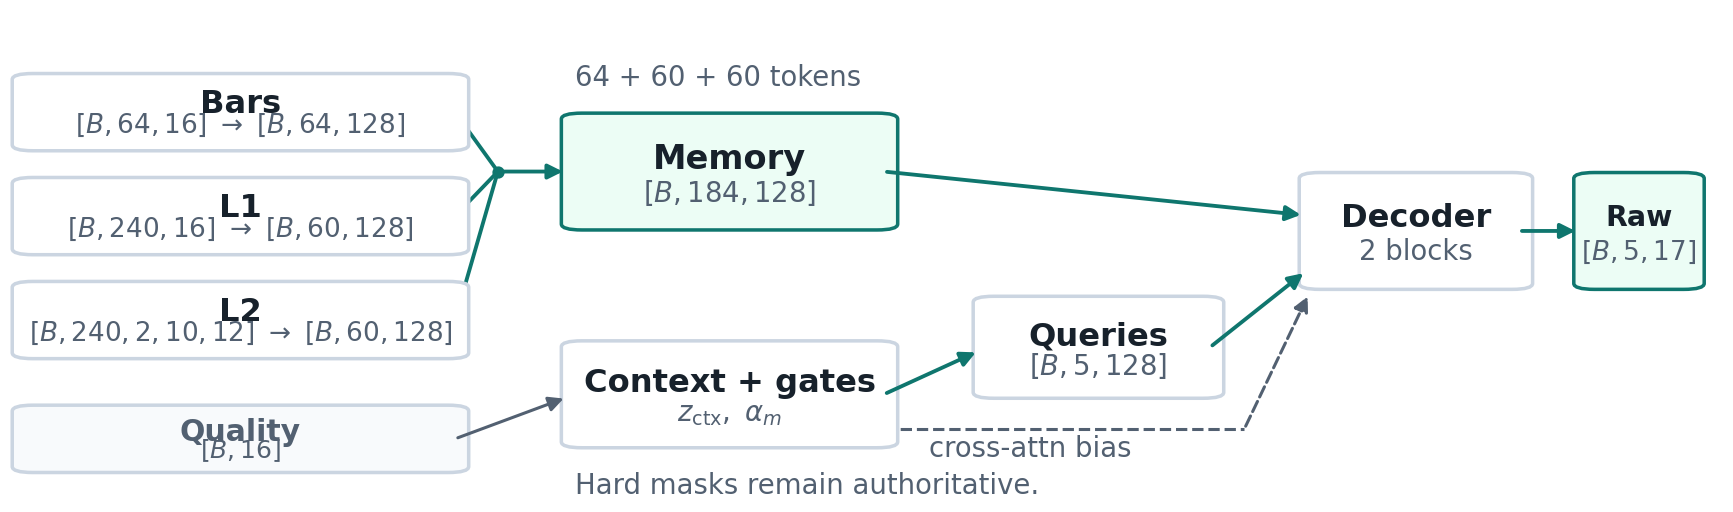
\includegraphics[width=0.98\textwidth]{architecture-shape-trace.png}
\caption{The three branches converge only after structural and temporal
encoding. Masks remain parallel to all value tensors.}
\label{fig:shape-trace}
\end{figure}

For one inference request, $B=1$. The main semantic path is therefore
\begin{equation}
\begin{split}
&[1,64,16],\ [1,240,16],\ [1,240,2,10,12],\ [1,16]\\
&\quad\longrightarrow [1,64,128],\ [1,60,128],\ [1,60,128]\\
&\quad\longrightarrow [1,184,128]\longrightarrow[1,5,128]
\longrightarrow[1,5,17].
\end{split}
\label{eq:batch-one-path}
\end{equation}

\section{Normalization, Time, and Structural Embeddings}

\subsection{Training-only robust scaling}

For each continuous feature $j$, valid training-partition values determine
\begin{equation}
\mu_j=\operatorname{median}_{\mathrm{train}}(x_j),\qquad
s_j=\max\!\left(1.4826\operatorname{MAD}_{\mathrm{train}}(x_j),s_{\min,j}\right),
\label{eq:scaler-fit}
\end{equation}
and the deployed transform is
\begin{equation}
z_j=\operatorname{clip}\!\left(\frac{x_j-\mu_j}{s_j},-8,8\right).
\label{eq:robust-scaling}
\end{equation}
Bounded shares, fractions, imbalances, and binary flags use identity scaling.
Invalid values are zeroed only after Equation~\eqref{eq:robust-scaling}; masks
are never scaled.

At a 500-ms grid time $g_t$, the eligible source observation is the latest
available observation not later than the grid time:
\begin{equation}
i^*(t)=\arg\max_i\{t_i^{\mathrm{available}}:
t_i^{\mathrm{available}}\le g_t\},
\label{eq:asof-sampling}
\end{equation}
subject to feed-epoch continuity, acceptance, and freshness. This as-of rule
preserves a fixed clock axis without future fill.

\subsection{Physical-time encoding}

Text position is not an adequate description of irregular market age. For
nonnegative age $a$, context maximum $a_{\max}$, and fixed scales
$\tau_1,\ldots,\tau_K$, define
\begin{equation}
\phi(a)=\left[
\frac{a}{a_{\max}},
\frac{\log(1+a)}{\log(1+a_{\max})},
\sin\frac{a}{\tau_1},\cos\frac{a}{\tau_1},\ldots,
\sin\frac{a}{\tau_K},\cos\frac{a}{\tau_K}
\right].
\label{eq:time-features}
\end{equation}
The branch-specific time embedding is
\begin{equation}
e_t(a)=W_{t,2}\SiLU(W_{t,1}\phi(a)+b_{t,1})+b_{t,2}.
\label{eq:time-mlp}
\end{equation}
Bars use $K=7$ and scales $(60,120,240,480,960,1920,3840)$ seconds.
Patched L1 and L2 use $K=8$ and scales
$(0.5,1,2,4,8,16,32,64)$ seconds. Bar slot-close ages are
$(3780,3720,\ldots,0)$ seconds; patch-end ages are
$(118,116,\ldots,0)$ seconds. These arrays are constants, not external inputs.

Every temporal token also receives a learned modality vector. An L2 level
state receives fixed-axis side and rank embeddings:
\begin{equation}
x_{b,t,s,r}^{2,(0)}=
W_{\mathrm{level}}z_{b,t,s,r}+b_{\mathrm{level}}
+e_s^{\mathrm{side}}+e_r^{\mathrm{rank}}.
\label{eq:l2-projection}
\end{equation}

\subsection{Learned relative-time bias}

Temporal attention head $j$ gives an eligible earlier key a learned recency
bias
\begin{equation}
\beta_{i\ell}^{(j)}=-\softplus(\gamma_j)
\log\!\left(1+\frac{t_i-t_\ell}{s_m}\right),
\qquad t_\ell\le t_i,
\label{eq:relative-time-bias}
\end{equation}
where $s_m=60$ seconds for bars and $s_m=2$ seconds for patched
microstructure. This is a soft content-independent prior. It does not replace
the causal or validity mask.

\section{The CHMT Primitive Block}

\subsection{RMS normalization}

For $x\in\R^d$, learned gain $g\in\R^d$, and $\epsilon>0$,
\begin{equation}
\RMSNorm(x)=g\odot
\frac{x}{\sqrt{d^{-1}\sum_{r=1}^{d}x_r^2+\epsilon}}.
\label{eq:rmsnorm}
\end{equation}
RMSNorm controls scale without subtracting a coordinate mean
\citep{zhang2019rms}.

\subsection{Q/K-normalized multi-head attention}

Let query states $U\in\R^{B\times n_q\times d}$ and memory states
$M\in\R^{B\times n_k\times d}$. For head $j$ with width $d_h=d/H_a$,
\begin{equation}
Q_j=UW_j^Q+b_j^Q,\quad
K_j=MW_j^K+b_j^K,\quad
V_j=MW_j^V+b_j^V.
\label{eq:qkv}
\end{equation}
Each query and key vector is RMS-normalized without a learned gain:
\begin{equation}
\bar q=\frac{q}{\sqrt{d_h^{-1}\lVert q\rVert_2^2+\epsilon}},
\qquad
\bar k=\frac{k}{\sqrt{d_h^{-1}\lVert k\rVert_2^2+\epsilon}}.
\label{eq:qk-normalization}
\end{equation}
With learned log-temperature $\theta_j$, optional time bias $\beta$, and
eligibility mask $\mathcal M$, define the cross-attention key-modality bias as
\(g_{m(\ell)}=\log(\alpha_{m(\ell)}+\epsilon)\); it is zero in attention
layers that do not use modality routing. The score is
\begin{equation}
s_{i\ell}^{(j)}=
e^{\theta_j}\frac{\bar q_i^{(j)\top}\bar k_\ell^{(j)}}{\sqrt{d_h}}
+\beta_{i\ell}^{(j)}
+g_{m(\ell)}+\mathcal M_{i\ell}.
\label{eq:attention-score}
\end{equation}
In temporal self-attention, $\mathcal M_{i\ell}$ permits a key only when it is
valid and no later than the query. In L2 within-snapshot attention there is no
causal triangle because all 20 positions coexist at one logical time. Decoder
cross-attention sees every valid historical memory key.

\subsection{Safe masked softmax}

Ordinary masked softmax is undefined when a query has no eligible key. Let
$m_{i\ell}\in\{0,1\}$ and $a_i=\bigvee_\ell m_{i\ell}$. Totalize the row
maximum as
\begin{equation}
s_i^{\max}=
\begin{cases}
\max_{\ell:m_{i\ell}=1}s_{i\ell},&a_i=1,\\
0,&a_i=0,
\end{cases}
\label{eq:safe-row-maximum}
\end{equation}
and define
\begin{equation}
r_{i\ell}=m_{i\ell}\exp(s_{i\ell}-s_i^{\max}),\qquad
p_{i\ell}=
\begin{cases}
r_{i\ell}/\sum_k r_{ik},&a_i=1,\\
0,&a_i=0.
\end{cases}
\label{eq:safe-softmax}
\end{equation}
Then every masked key has exactly zero weight, every nonempty eligible row sums
to one, and every empty row returns zero without a nonfinite intermediate in
the reference path. At training time, attention-weight dropout is applied after
the safe softmax; at inference it is the identity. Multi-head output is
\begin{equation}
\Attn(U,M)=\operatorname{Concat}_{j=1}^{H_a}
(\operatorname{Dropout}(P_j)V_j)W^O+b^O.
\label{eq:attention-output}
\end{equation}

\subsection{SwiGLU and residual update}

The feed-forward sublayer is
\begin{equation}
\FFN(x)=W_o\!\left[
\SiLU(W_gx+b_g)\odot(W_ux+b_u)
\right]+b_o,
\label{eq:swiglu}
\end{equation}
with main widths $128\rightarrow256\rightarrow128$ and level widths
$32\rightarrow64\rightarrow32$ \citep{shazeer2020}. For encoder input $x$,
let $\bar x=\RMSNorm_a(x)$. The pre-normalized LayerScale updates are
\begin{align}
u&=x+\lambda_a\odot
\operatorname{Dropout}(\Attn(\bar x,\bar x)),\nonumber\\
z&=u+\lambda_f\odot
\operatorname{Dropout}(\FFN(\RMSNorm_f(u))).
\label{eq:encoder-residual}
\end{align}
Both $\lambda_a$ and $\lambda_f$ are learned $d$-vectors initialized to 0.1.
The query-validity mask multiplies $z$ after the residual path. Dropout is 0.10
during training and disabled at inference.

\section{Three Structure-Preserving Encoders}

\subsection{Bar encoder: 64 unpatched tokens}

Each normalized bar row is independently projected from 16 to 128 dimensions,
then receives its modality and physical-time embeddings:
\begin{equation}
X^{b,(0)}=(X^bW_b+b_b)+E_t^b+e^b_{\mathrm{mod}}.
\label{eq:bar-embedding}
\end{equation}
Three causal CHMT blocks preserve the shape $[B,64,128]$. The bar branch is
\emph{not patched}: the final memory contains all 64 minute states. Its causal
triangle ensures every intermediate state summarizes only its own prefix.

\subsection{L1 encoder: four-frame causal patches}

L1 rows are projected to width 128. Four consecutive 500-ms frames form a
non-overlapping two-second patch. With projected frame $x_j$, validity $m_j$,
and learned within-patch offset $e_j^{\mathrm{patch}}$, the pooling score and
output are
\begin{align}
\widetilde x_j&=x_j+e_j^{\mathrm{patch}},\qquad j\in\{0,1,2,3\},\nonumber\\
r_j&=w_2^\top\tanh(W_1\widetilde x_j+b_1)+b_2,\nonumber\\
\pi_j&=\SafeSoftmax_j(r_j;m_j),\qquad
p=\sum_{j=0}^{3}\pi_j\widetilde x_j.
\label{eq:patch-pool}
\end{align}
An all-invalid patch returns a zero vector and false mask. Reshaping and pooling
give
\begin{equation}
[B,240,128]\rightarrow[B,60,4,128]\rightarrow[B,60,128].
\label{eq:l1-patch-shape}
\end{equation}
Patch-end time and modality embeddings are added, followed by three independent
causal CHMT blocks.

\subsection{L2 encoder: side/rank first, time second}

\begin{figure}[!htbp]
\centering
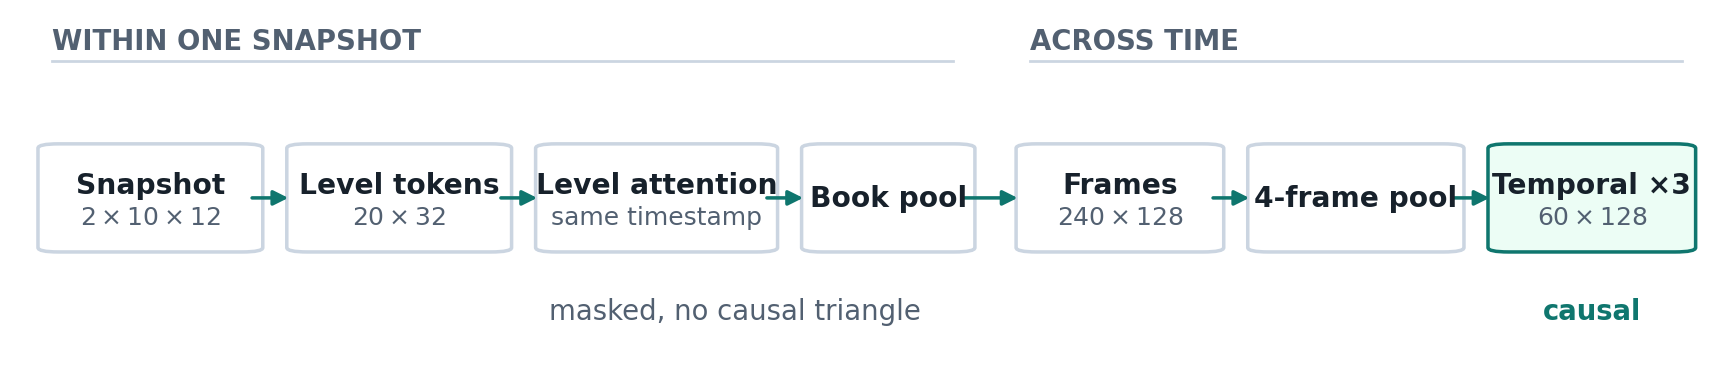
\includegraphics[width=0.98\textwidth]{architecture-l2-hierarchy.png}
\caption{The L2 hierarchy separates same-time book geometry from temporal
evolution. The level block is noncausal across the 20 simultaneous cells; the
later temporal blocks are causal.}
\label{fig:l2-hierarchy}
\end{figure}

For every one of 240 grid times, fixed side and rank axes flatten as
\begin{equation}
[B,240,2,10,12]\rightarrow[B\cdot240,20,12]
\rightarrow[B\cdot240,20,32].
\label{eq:l2-flatten}
\end{equation}
Equation~\eqref{eq:l2-projection} supplies level states. One masked, noncausal
level CHMT block models interactions among the contemporaneous bid/ask ranks.
For learned book query $q_{\mathrm{book}}\in\R^{32}$, pool weights and the
depth-frame token are
\begin{align}
a_{b,t,s,r}&=\SafeSoftmax_{s,r}\!\left(
\frac{q_{\mathrm{book}}^\top\RMSNorm(x_{b,t,s,r})}{\sqrt{32}};
m^{2,L}_{b,t,s,r}\right),\nonumber\\
d_{b,t}&=W_d\sum_{s=0}^{1}\sum_{r=0}^{9}
a_{b,t,s,r}x_{b,t,s,r}+b_d\in\R^{128}.
\label{eq:book-pool}
\end{align}
This produces $[B,240,128]$. The independently parameterized four-frame pool
reduces it to $[B,60,128]$, and three causal temporal CHMT blocks encode its
two-minute evolution.

The hierarchy avoids a flat 4,800-token temporal sequence. A flat attention
matrix would contain $4{,}800^2=23{,}040{,}000$ scores per head and layer,
while also mixing same-snapshot rank structure with temporal order.

\section{Quality-Aware Fusion}

Let $M_b\in\R^{B\times64\times128}$,
$M_1\in\R^{B\times60\times128}$, and
$M_2\in\R^{B\times60\times128}$ denote encoded memories and let
$m_m$ denote their token masks. The latest valid index and summary are
\begin{equation}
t_m^*(b)=\max\{t:m_{m,b,t}=1\},\qquad
s_{m,b}=M_{m,b,t_m^*(b)},
\label{eq:latest-valid}
\end{equation}
with a zero summary and hard availability $a_{m,b}=0$ when the set is empty.
The quality MLP is
\begin{equation}
c_q=W_{q,2}\SiLU(W_{q,1}q+b_{q,1})+b_{q,2}\in\R^{B\times128}.
\label{eq:quality-mlp}
\end{equation}
Each modality has an independent gate:
\begin{align}
\widetilde g_m&=a_m\sigmoid\!\left(
w_{m,2}^{\top}\SiLU(W_{m,1}[s_m;c_q]+b_{m,1})+b_{m,2}
\right),\nonumber\\
\alpha_m&=\frac{\widetilde g_m}{\sum_n\widetilde g_n+\epsilon},\qquad
z_{\mathrm{ctx}}=\RMSNorm\!\left(c_q+\sum_m\alpha_ms_m\right).
\label{eq:quality-gates}
\end{align}
The historical memory is a concatenation, not a pooled summary:
\begin{equation}
M=[M_b;M_1;M_2]\in\R^{B\times184\times128}.
\label{eq:fused-memory}
\end{equation}
Decoder cross-attention receives $\log(\alpha_m+\epsilon)$ as the score bias
for keys from modality $m$. The gate does not also multiply memory values.
Hard-masked branches remain ineligible regardless of learned gate values. If
all three modalities are unavailable, the host abstains before model execution.

\begin{figure}[!htbp]
\centering
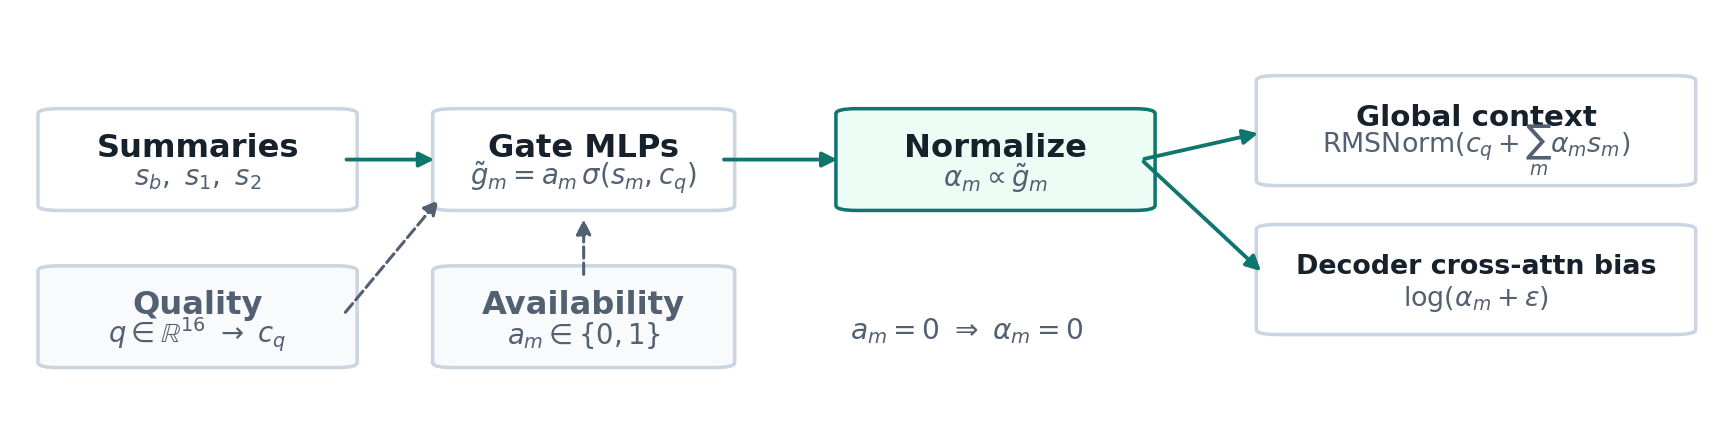
\includegraphics[width=0.98\textwidth]{architecture-quality-gates.png}
\caption{Hard availability bounds the learned reliability gates. A soft gate
may downweight available evidence but cannot restore a masked branch.}
\label{fig:quality-gating}
\end{figure}

\section{Direct Five-Horizon Decoder}

For horizon $h\in\{1,\ldots,5\}$, let $e_h\in\R^{128}$ be a learned base
query. With shared horizon MLP output \(u_h\) and context projection
\(W_{\mathrm{ctx}}\), initialize
\begin{align}
\xi_h&=[h/5,\ \log(1+h),\ h\Delta],\nonumber\\
u_h&=W_{h,2}\SiLU(W_{h,1}\xi_h+b_{h,1})+b_{h,2},\nonumber\\
Q_h^{(0)}&=e_h+W_{\mathrm{ctx}}z_{\mathrm{ctx}}+b_{\mathrm{ctx}}+u_h.
\label{eq:horizon-query}
\end{align}
Stacking gives $Q^{(0)}\in\R^{B\times5\times128}$. Decoder block $\ell$
performs three residual updates in a fixed order:
\begin{align}
A^{(\ell)}&=Q^{(\ell)}+\lambda_s^{(\ell)}\odot
\Attn_s(\RMSNorm(Q^{(\ell)}),\RMSNorm(Q^{(\ell)})),\nonumber\\
C^{(\ell)}&=A^{(\ell)}+\lambda_c^{(\ell)}\odot
\Attn_c(\RMSNorm(A^{(\ell)}),M),\nonumber\\
Q^{(\ell+1)}&=C^{(\ell)}+\lambda_f^{(\ell)}\odot
\FFN(\RMSNorm(C^{(\ell)})),\qquad \ell\in\{0,1\}.
\label{eq:decoder-block}
\end{align}
Dropout surrounds each residual branch during training and is omitted from
Equation~\eqref{eq:decoder-block} for readability. Horizon self-attention is
noncausal because all five queries are constructed at the same decision time.
No predicted horizon is used as input to another; all five forecasts are direct
functions of the same historical memory. Each decoder block has exactly three
learned RMSNorm gains---one before query self-attention, one before the
cross-attention query, and one before the feed-forward layer. No additional
learned RMSNorm is applied to memory \(M\) inside cross-attention.

\section{Raw Output, Ordered Quantiles, and Physical Units}

\subsection{Exact 17-slot map}

The shared head is
\begin{equation}
R=Q^{(2)}W_R+b_R\in\R^{B\times5\times17}.
\label{eq:raw-head}
\end{equation}
It emits raw parameters, not already reconstructed quantiles. For target
$k\in\{0,\ldots,4\}$,
\begin{equation}
(r_{h,k},a_{h,k},b_{h,k})=
(R_{h,3k},R_{h,3k+1},R_{h,3k+2}).
\label{eq:raw-index}
\end{equation}

\begin{table}[!htbp]
\centering
\small
\begin{tabularx}{\textwidth}{@{}c l l Y@{}}
\toprule
\textbf{Slots} & \textbf{Target} & \textbf{Raw meaning} & \textbf{Semantic meaning after transforms}\\
\midrule
0--2 & total POC & center, lower-gap logit, upper-gap logit & q10/q50/q90 tick offset\\
3--5 & buy POC & center, lower-gap logit, upper-gap logit & conditional q10/q50/q90 tick offset\\
6--8 & sell POC & center, lower-gap logit, upper-gap logit & conditional q10/q50/q90 tick offset\\
9--11 & log-volume residual & center, lower-gap logit, upper-gap logit & q10/q50/q90 future volume\\
12--14 & delta fraction & center, lower-gap logit, upper-gap logit & bounded q10/q50/q90 fraction\\
15 & buy POC presence & logit & probability that an eligible buy POC exists\\
16 & sell POC presence & logit & probability that an eligible sell POC exists\\
\bottomrule
\end{tabularx}
\caption{Target-major raw-head indexing for each horizon.}
\label{tab:raw-index}
\end{table}

The two presence probabilities are
\begin{equation}
\widehat p_h^{\mathrm{buy}}=\sigmoid(R_{h,15}),\qquad
\widehat p_h^{\mathrm{sell}}=\sigmoid(R_{h,16}).
\label{eq:presence-probabilities}
\end{equation}
They indicate target existence under the label contract. They do not indicate
trade direction.

\subsection{Noncrossing quantile construction}

For every $(h,k)$, define normalized quantiles
\begin{equation}
\widetilde Q_{h,k,0.50}=r_{h,k},\qquad
\widetilde Q_{h,k,0.10}=r_{h,k}-\softplus(a_{h,k}),\qquad
\widetilde Q_{h,k,0.90}=r_{h,k}+\softplus(b_{h,k}).
\label{eq:ordered-head}
\end{equation}
The delta-fraction target uses its bounded semantic value inside the loss. Define
the post-head prediction
\begin{equation}
Q^\star_{h,k,\tau}=
\begin{cases}
\widetilde Q_{h,k,\tau},&k\in\{0,1,2,3\},\\
\tanh(\widetilde Q_{h,4,\tau}),&k=4.
\end{cases}
\label{eq:semantic-quantiles}
\end{equation}

\begin{proposition}[Order preservation]
Equation~\eqref{eq:ordered-head} satisfies
$\widetilde Q_{h,k,0.10}<\widetilde Q_{h,k,0.50}<
\widetilde Q_{h,k,0.90}$ over exact real
arithmetic. Any nondecreasing inverse transformation preserves weak order.
\end{proposition}
\begin{proof}
$\softplus(x)=\log(1+e^x)>0$ for every finite $x$. Therefore
$r-\softplus(a)<r<r+\softplus(b)$. If $f$ is nondecreasing and
$x_1<x_2<x_3$, then $f(x_1)\le f(x_2)\le f(x_3)$. This applies to affine
inverse scaling, the exponential volume map, and $\tanh$ for delta fraction.
Finite-precision saturation may turn a strict inequality into equality but
cannot reverse it.
\end{proof}

\subsection{Inverse normalization and reconstruction}

For price and log-volume targets, first reverse
Equation~\eqref{eq:target-normalization} independently for every $(h,k,\tau)$:
\begin{equation}
\widehat y_{h,k,\tau}=\mu^Y_{h,k}
+s^Y_{h,k}Q^\star_{h,k,\tau},\qquad k\in\{0,1,2,3\}.
\label{eq:inverse-target-scale}
\end{equation}
The primitive physical outputs are then
\begin{align}
\widehat P_{h,k,\tau}&=p_{\mathrm{ref}}
+\delta_p\widehat y_{h,k,\tau}, && k\in\{0,1,2\},\nonumber\\
\widehat V_{h,\tau}&=\max\!\left(0,
\exp(\ell_{\mathrm{ref}}+\widehat y_{h,3,\tau})-1\right),\nonumber\\
\widehat f_{D,h,\tau}&=Q^\star_{h,4,\tau}.
\label{eq:physical-reconstruction}
\end{align}
Prices are snapped to the instrument tick only after reconstruction. Finite
values, quantile order, nonnegative volume, bounded delta fraction, presence
decisions, and the five-horizon shape are checked before release.

The output contains three ordered marginal quantile forecasts for each of five
targets at each of five horizons. It is not a full probability distribution or
a coherent joint sample path. The q10--q90 pair is a nominal central 80\% band;
its empirical coverage is not guaranteed without separate calibration. In
particular, multiplying a volume quantile by a delta-fraction quantile does not
produce a valid quantile of raw delta.

\subsection{Worked synthetic output-reconstruction example}

Consider one syntactically valid inference request: value tensors and masks
have the batch-one shapes in Table~\ref{tab:external-inputs}; the L1 and L2
windows contain 240 grid rows; the bar window contains 64 slots. Suppose the
head produces, for one horizon and total-POC target,
\begin{equation}
(r,a,b)=(0.20,-0.50,0.10).
\label{eq:worked-raw}
\end{equation}
Since $\softplus(-0.50)=0.4741$ and
$\softplus(0.10)=0.7444$, Equation~\eqref{eq:ordered-head} gives
\begin{equation}
(\widetilde Q_{0.10},\widetilde Q_{0.50},\widetilde Q_{0.90})
=(-0.2741,0.2000,0.9444).
\label{eq:worked-quantiles}
\end{equation}
If the frozen target scaler for that cell has $\mu^Y=0$ and $s^Y=4$ ticks,
the unnormalized offsets are
\begin{equation}
(-1.0964,0.8000,3.7776)\ \text{ticks}.
\label{eq:worked-ticks}
\end{equation}
With $p_{\mathrm{ref}}=100$ and $\delta_p=0.5$, the pre-snapping physical
POCs are $(99.4518,100.4000,101.8888)$. This is an illustrative arithmetic
trace, not a reported model prediction. If the same horizon's presence logits
were $(2,-1)$, their probabilities would be
$(\sigmoid(2),\sigmoid(-1))=(0.8808,0.2689)$.

\section{Training Objective}

\subsection{Pinball loss and its quantile condition}

For level $\tau\in(0,1)$, outcome $y$, prediction $q$, and residual $u=y-q$,
the pinball loss is
\begin{equation}
\rho_\tau(u)=u(\tau-\I\{u<0\})
=\max\{\tau u,(\tau-1)u\}.
\label{eq:pinball}
\end{equation}

\begin{derivationbox}{Why the minimizer is a conditional quantile}
For conditional distribution $F_{Y\mid X}$, let
$R(q\mid X)=\E[\rho_\tau(Y-q)\mid X]$. Away from atoms,
\begin{align}
\frac{\partial R}{\partial q}
&=(1-\tau)\Pr(Y<q\mid X)-\tau\Pr(Y>q\mid X)\nonumber\\
&=F_{Y\mid X}(q)-\tau.
\label{eq:pinball-derivative}
\end{align}
A stationary minimum therefore satisfies $F_{Y\mid X}(q)=\tau$. At an atom,
the subgradient condition is $F(q^-)\le\tau\le F(q)$, which is the standard
quantile definition. The property pertains to the target defined in
Equation~\eqref{eq:targets}; it does not change that target's semantics.
\end{derivationbox}

Let horizon weights $w_h=h^{-1/2}$, target weights
$v=(1,1,1,0.5,0.5)$, quantile levels
$\mathcal T=\{0.1,0.5,0.9\}$, and target mask $m^Y_{b,h,k}$. The normalized
primary loss is
\begin{equation}
\mathcal L_Q=
\frac{\sum_{b,h,k,\tau}m^Y_{b,h,k}w_hv_k
\rho_\tau(\widetilde y_{b,h,k}-Q^\star_{b,h,k,\tau})}
{\sum_{b,h,k,\tau}m^Y_{b,h,k}w_hv_k+\epsilon}.
\label{eq:weighted-pinball}
\end{equation}

\subsection{Median stabilization and presence loss}

For normalized median residual $r$ and threshold $\delta=1$,
\begin{equation}
H_\delta(r)=
\begin{cases}
\tfrac12r^2,&|r|\le\delta,\\
\delta(|r|-\tfrac12\delta),&|r|>\delta.
\end{cases}
\label{eq:huber}
\end{equation}
The masked, weighted median loss is
\begin{equation}
\mathcal L_H=
\frac{\sum_{b,h,k}m^Y_{b,h,k}w_hv_k
H_1(\widetilde y_{b,h,k}-Q^\star_{b,h,k,0.5})}
{\sum_{b,h,k}m^Y_{b,h,k}w_hv_k+\epsilon}.
\label{eq:median-huber}
\end{equation}

For presence label $z\in\{0,1\}$ and logit $\eta$, stable binary
cross-entropy is
\begin{equation}
\operatorname{BCE}(\eta,z)=
\max(\eta,0)-\eta z+\log(1+e^{-|\eta|}).
\label{eq:bce-scalar}
\end{equation}
With an independent presence-validity mask $m^P$, define
\begin{equation}
\mathcal L_P=
\frac{\sum_{b,h,s}m^P_{b,h,s}
\operatorname{BCE}(\eta_{b,h,s},z_{b,h,s})}
{\sum_{b,h,s}m^P_{b,h,s}+\epsilon}.
\label{eq:presence-loss}
\end{equation}

The same shared head applied after decoder block one supplies an auxiliary
deep-supervision loss. For optimizer-step fraction $u\in[0,1]$,
\begin{equation}
\lambda_{\mathrm{aux}}(u)=
\begin{cases}
0.25,&u\le0.60,\\
0.25-\dfrac{0.20}{0.30}(u-0.60),&0.60<u<0.90,\\
0.05,&u\ge0.90.
\end{cases}
\label{eq:aux-schedule}
\end{equation}
With $\mathcal L_{\mathrm{base}}=\mathcal L_Q+0.25\mathcal L_H
+0.20\mathcal L_P$, the total objective is
\begin{equation}
\mathcal L=\mathcal L_{\mathrm{base}}^{\mathrm{final}}
+\lambda_{\mathrm{aux}}(u)\mathcal L_{\mathrm{base}}^{\mathrm{block\ 1}}.
\label{eq:total-loss}
\end{equation}

\section{Parameter and Attention-Work Derivation}

\subsection{Primitive formulas}

A biased linear map $a\rightarrow b$ contains
\begin{equation}
P_{\mathrm{linear}}(a,b)=ab+b
\label{eq:linear-params}
\end{equation}
parameters. A SwiGLU map $d\rightarrow f\rightarrow d$ has two input
projections and one output projection:
\begin{equation}
P_{\mathrm{SwiGLU}}(d,f)
=2(df+f)+(fd+d)=3df+2f+d.
\label{eq:swiglu-params}
\end{equation}

For a main temporal CHMT block with $d=128$, $f=256$, and four heads,
\begin{align}
P_{\mathrm{attn}}&=4(d^2+d)=66{,}048,\nonumber\\
P_{\mathrm{SwiGLU}}&=3df+2f+d=98{,}944,\nonumber\\
P_{\mathrm{norm+scale}}&=2d+2d=512,\nonumber\\
P_{\mathrm{temperature+time}}&=4+4=8,\nonumber\\
P_{\mathrm{temporal\ block}}&=165{,}512.
\label{eq:main-block-params}
\end{align}
There are nine such blocks, so their total is
$9\times165{,}512=1{,}489{,}608$.

For the L2 level block, $d=32$, $f=64$, and four heads. It has
\begin{equation}
4(32^2+32)+(3\cdot32\cdot64+2\cdot64+32)
+4\cdot32+4=10{,}660,
\label{eq:level-block-params}
\end{equation}
where the final four scalars are head temperatures; level attention has no
elapsed-time decay.

One decoder block contains self-attention, cross-attention, one SwiGLU, three
RMSNorm gains, three LayerScale vectors, and eight head temperatures:
\begin{equation}
2\cdot66{,}048+98{,}944+3\cdot128+3\cdot128+8
=231{,}816.
\label{eq:decoder-params}
\end{equation}
Two blocks therefore contain 463,632 parameters.

\subsection{Literal component ledger}

\begin{table}[H]
\centering
\small
\begin{tabular}{@{}lr@{}}
\toprule
\textbf{Component} & \textbf{Trainable parameters}\\
\midrule
Bar, L1, and L2-level projections & 4,768\\
Quality MLP & 18,688\\
Bar time MLP & 4,768\\
L1 patch-time MLP & 4,832\\
L2 patch-time MLP & 4,832\\
Three modality embeddings & 384\\
L2 side and rank embeddings & 384\\
L2 level CHMT block & 10,660\\
Book query, pool norm, and 32-to-128 projection & 4,288\\
L1/L2 within-patch embeddings and pool MLPs & 9,346\\
Nine temporal CHMT blocks & 1,489,608\\
Two decoder blocks & 463,632\\
Three modality-gate MLPs & 49,539\\
Fusion norm and context projection & 16,640\\
Horizon queries and horizon MLP & 4,992\\
Shared 128-to-17 output head & 2,193\\
\midrule
\textbf{Total} & \textbf{2,089,554}\\
\bottomrule
\end{tabular}
\caption{Exact trainable-parameter ledger. The total includes 36 learned
per-head Q/K temperatures in the nine temporal blocks.}
\label{tab:parameter-ledger}
\end{table}

Several rows can be checked directly. The quality MLP is
\begin{equation}
P_{q}=(16\cdot128+128)+(128^2+128)=18{,}688.
\label{eq:quality-params}
\end{equation}
Each modality gate is $256\rightarrow64\rightarrow1$:
\begin{equation}
P_{\mathrm{gate}}=(256\cdot64+64)+(64\cdot1+1)=16{,}513,
\label{eq:gate-params}
\end{equation}
and $3P_{\mathrm{gate}}=49{,}539$. The shared head contains
$128\cdot17+17=2{,}193$ parameters. The two patch modules each contain four
128-vectors plus a $128\rightarrow32\rightarrow1$ scoring MLP:
\begin{equation}
P_{\mathrm{patch}}=4\cdot128+(128\cdot32+32)+(32+1)=4{,}673,
\label{eq:patch-params}
\end{equation}
giving 9,346 across L1 and L2.

\subsection{Why dense attention is small here}

Per layer and head, all temporal score matrices contain
\begin{equation}
64^2+60^2+60^2=11{,}296
\label{eq:encoder-score-count}
\end{equation}
entries. Across three layers and four heads, that is
\begin{equation}
3\cdot4\cdot11{,}296=135{,}552.
\label{eq:all-encoder-scores}
\end{equation}
Two decoder cross-attention layers add
\begin{equation}
2\cdot4\cdot5\cdot184=7{,}360
\label{eq:decoder-score-count}
\end{equation}
entries. For one batch element, the single level block across all 240
snapshots contributes
\begin{equation}
240\cdot4\cdot20^2=384{,}000
\label{eq:level-score-count}
\end{equation}
entries, and two decoder self-attention layers contribute
\begin{equation}
2\cdot4\cdot5^2=200.
\label{eq:decoder-self-score-count}
\end{equation}
The complete multi-head Q/K attention-score count for one forward pass is
therefore
\begin{equation}
135{,}552+384{,}000+7{,}360+200=527{,}112.
\label{eq:total-score-count}
\end{equation}
Book-query pooling evaluates another \(240\cdot20=4{,}800\) scalar
compatibility scores, and the two patch pools evaluate
\(2\cdot60\cdot4=480\) MLP scores; neither is a multi-head Q/K matrix. At
these sequence lengths, dense temporal attention score storage is modest;
the repeated projections, feed-forward layers, and 240 snapshot-level passes
dominate arithmetic.

\section{Reference Forward Pass and Inference Contract}

The complete computation is the following ordered map:
\begin{enumerate}
  \item validate all external shapes, dtypes, finite values, and the nested L2
  mask invariant in Equation~\eqref{eq:nested-mask};
  \item robust-scale valid numeric inputs with frozen training statistics and
  zero invalid rows;
  \item project bars and L1, and project each L2 side--rank cell with internal
  side/rank embeddings;
  \item run one level CHMT block and book-query pool for every L2 snapshot;
  \item pool each nonoverlapping group of four L1 and L2 frames; do not patch
  bars;
  \item add modality and physical-time embeddings, then run three causal CHMT
  blocks independently on each branch;
  \item extract latest-valid summaries, compute quality context and the three
  hard-aware gates, and concatenate the 184 memory tokens;
  \item construct five horizon queries, then apply two decoder blocks in the
  self-attention $\rightarrow$ cross-attention $\rightarrow$ SwiGLU order;
  \item map the five final states to $[B,5,17]$ raw values;
  \item construct ordered quantiles and presence probabilities, reverse target
  normalization, reconstruct physical values, snap prices, and apply all output
  invariants.
\end{enumerate}

The raw graph returns only $R$ from Equation~\eqref{eq:raw-head}. A serving
wrapper binds the model bytes to feature-schema, scaler, target-transform,
calibration, tick-rule, and model-version hashes. A valid inference result must
satisfy
\begin{equation}
\begin{gathered}
R\in\R^{1\times5\times17},\qquad
Q_{0.10}\le Q_{0.50}\le Q_{0.90},\\
\widehat V\ge0,\qquad -1\le\widehat f_D\le1,\qquad
0\le\widehat p^{\mathrm{side}}\le1.
\end{gathered}
\label{eq:output-invariants}
\end{equation}
Any schema mismatch, stale reference, all-modality mask, nonfinite result, or
invariant violation yields a reason-coded abstention rather than a partial
forecast.

\section{Related Design Choices}

CHMT-Q uses dense attention because its temporal sequences contain only 64 or
60 tokens. Relative elapsed-time bias adapts relative-position attention
\citep{shaw2018} to physical clock differences. Patch pooling is related to
PatchTST's use of temporal patches \citep{nie2023}, but CHMT-Q jointly embeds
interacting numeric fields rather than enforcing channel independence. Direct
horizon queries resemble multi-horizon decoding in Temporal Fusion Transformer
\citep{lim2021}; the hard masks and explicit quality routes are specific to the
present contract.

The depth hierarchy follows the broad lesson of DeepLOB and later LOB models:
same-snapshot spatial structure and across-time evolution deserve separate
processing \citep{deepLOB2019,wallbridge2020,zhang2021lob}. Unlike a flattened
book, CHMT-Q lets rank and side interact before reducing one snapshot to one
temporal frame. Its ordered head uses quantile regression, whose proper-score
interpretation is established by the pinball-loss result
\citep{gneiting2007}. The marginals could later be calibrated on a dedicated
calibration partition, for example by conformalized quantile methods under
their stated assumptions \citep{romano2019}; calibration is not implicit in
the architectural ordering guarantee.

\section{Implementation Status and Research Boundary}

The tensor shapes, primitive blocks, and 2,089,554-parameter count in this
paper correspond to the implemented CHMT-Q model and its frozen architecture
ledger. The model has been trained in an offline research study. It has no
established live-terminal integration or production-deployment status. This
mechanics paper reports neither an independent performance estimate nor an
economic result, and it makes no claim of executable edge or profitability.
Existing evidence does not establish useful conditional medians, executable
edge, or profitability. The artifact remains research-only and non-promotable.

The model is a forecast provider. It does not choose side, position size,
leverage, stop, venue, or order type. Any downstream consumer must preserve the
cutoff and scaler contracts, distinguish a forecast from realized footprint
data, and evaluate decision utility, costs, risk, and operational behavior in
its own protocol.

Raw exchange archives, compiled tensors, prediction tapes, model weights, and
resumable checkpoints are not included in the paper source package. Their
distribution requires a separate provenance, licensing, privacy, and release
decision. The source bundle contains the manuscript and the figures necessary
to reproduce this document; it is not a public end-to-end reproduction package.

\section{Conclusion}

CHMT-Q maps four masked numeric market views to five direct probabilistic
forecasts through a structure-preserving Transformer. Its defining operations
are explicit: 64 unpatched bar tokens; 60 pooled L1 tokens; 60 hierarchical L2
tokens; a 184-token gated memory; five horizon queries; and a 17-value raw head
at each horizon. The output map is equally explicit: five center/gap triplets
become ordered q10/q50/q90 marginals, two logits become side-POC presence
probabilities, and frozen inverse transforms recover physical price, volume,
and delta-fraction units. Every step retains an authoritative validity mask.

The detailed derivations make the model auditable at the level where numeric
market systems most often become ambiguous: which observation is legal at the
cutoff, what every axis means, which values can attend, what each raw output
slot encodes, and which transformation returns it to physical units. Those
contracts define CHMT-Q more precisely than the word ``Transformer'' alone.

\appendix

\section{Compact Symbol Table}

\begin{longtable}{@{}p{3.2cm}p{12.6cm}@{}}
\caption{Principal notation.}\label{tab:notation}\\
\toprule
\textbf{Symbol} & \textbf{Meaning}\\
\midrule
\endfirsthead
\toprule
\textbf{Symbol} & \textbf{Meaning}\\
\midrule
\endhead
$B$ & batch size; fixed to one for exported inference\\
$t_c$ & wall-clock feature boundary and first target-interval opening\\
$c=t_c^{-}$ & logical total-order cutoff immediately before the target-open phase\\
$\kappa_i$ & deterministic total-order key of captured record \(i\)\\
$\mathcal F_c$ & information available by cutoff\\
$h,H$ & horizon index and horizon count; $H=5$\\
$k$ & target index; total POC, buy POC, sell POC, log-volume residual, delta fraction\\
$p_{\mathrm{ref}}$ & fresh causal reference price\\
$\delta_p$ & instrument tick size\\
$\ell_{\mathrm{ref}}$ & causal trailing log-volume reference\\
$d,d_h,d_{\mathrm{ff}}$ & model, attention-head, and feed-forward widths\\
$m$ & Boolean validity or attention-eligibility mask\\
$\alpha_m$ & normalized quality gate for modality $m$\\
$z_{\mathrm{ctx}}$ & fused 128-dimensional quality and modality context\\
$r_{h,k}$ & raw center parameter for horizon \(h\), target \(k\)\\
$Q_\tau$ & conditional quantile at level $\tau$\\
$\rho_\tau$ & pinball loss at level $\tau$\\
$\theta$ & all trainable model parameters\\
\bottomrule
\end{longtable}

\section{Mask Algebra}

For a temporal query $i$ and key $\ell$, the encoder eligibility indicator is
\begin{equation}
e_{i\ell}=m_i^{\mathrm{query}}m_\ell^{\mathrm{key}}
\I\{t_\ell\le t_i\}.
\label{eq:temporal-eligibility}
\end{equation}
For L2 level attention inside snapshot $t$,
\begin{equation}
e_{(s,r),(s',r')}=m^{2,L}_{t,s,r}m^{2,L}_{t,s',r'},
\label{eq:level-eligibility}
\end{equation}
because all cells share one timestamp. For decoder cross-attention,
\begin{equation}
e_{h,\ell}=m_\ell^{\mathrm{memory}},
\label{eq:cross-eligibility}
\end{equation}
and the learned quality gate appears only as a finite score bias. These three
relations separate temporal causality, structural coexistence, and reliability
routing.

\section{Source-Package Manifest}

The submission archive contains this LaTeX source and the three referenced PNG
figures. It intentionally excludes raw or compiled market data, prediction
tapes, weights, checkpoints, credentials, and licensed feeds. The document is
independently compilable with the figure directories preserved.

\begin{thebibliography}{13}

\bibitem{vaswani2017}
A.~Vaswani et al.
\newblock Attention is all you need.
\newblock \emph{Advances in Neural Information Processing Systems}, 30, 2017.
\newblock \url{https://arxiv.org/abs/1706.03762}.

\bibitem{shaw2018}
P.~Shaw, J.~Uszkoreit, and A.~Vaswani.
\newblock Self-attention with relative position representations.
\newblock \emph{NAACL-HLT}, pages 464--468, 2018.
\newblock \url{https://doi.org/10.18653/v1/N18-2074}.

\bibitem{zhang2019rms}
B.~Zhang and R.~Sennrich.
\newblock Root mean square layer normalization.
\newblock \emph{Advances in Neural Information Processing Systems}, 32, 2019.
\newblock \url{https://arxiv.org/abs/1910.07467}.

\bibitem{shazeer2020}
N.~Shazeer.
\newblock GLU variants improve Transformer.
\newblock Technical report, 2020.
\newblock \url{https://arxiv.org/abs/2002.05202}.

\bibitem{nie2023}
Y.~Nie et al.
\newblock A time series is worth 64 words: Long-term forecasting with
Transformers.
\newblock \emph{International Conference on Learning Representations}, 2023.
\newblock \url{https://arxiv.org/abs/2211.14730}.

\bibitem{lim2021}
B.~Lim, S.~O. Arik, N.~Loeff, and T.~Pfister.
\newblock Temporal fusion Transformers for interpretable multi-horizon time
series forecasting.
\newblock \emph{International Journal of Forecasting}, 37(4):1748--1764, 2021.
\newblock \url{https://doi.org/10.1016/j.ijforecast.2021.03.012}.

\bibitem{deepLOB2019}
Z.~Zhang, S.~Zohren, and S.~Roberts.
\newblock DeepLOB: Deep convolutional neural networks for limit order books.
\newblock \emph{IEEE Transactions on Signal Processing}, 67(11):3001--3012,
2019.
\newblock \url{https://doi.org/10.1109/TSP.2019.2907260}.

\bibitem{wallbridge2020}
J.~Wallbridge.
\newblock Transformers for limit order books.
\newblock Technical report, 2020.
\newblock \url{https://arxiv.org/abs/2003.00130}.

\bibitem{zhang2021lob}
Z.~Zhang and S.~Zohren.
\newblock Multi-horizon forecasting for limit order books: Novel deep learning
approaches and hardware acceleration using intelligent processing units.
\newblock Technical report, 2021.
\newblock \url{https://arxiv.org/abs/2105.10430}.

\bibitem{ntakaris2018}
A.~Ntakaris et al.
\newblock Benchmark dataset for mid-price forecasting of limit order book data
with machine learning methods.
\newblock \emph{Journal of Forecasting}, 37(8):852--866, 2018.
\newblock \url{https://doi.org/10.1002/for.2543}.

\bibitem{kolm2023}
P.~N. Kolm, J.~Turiel, and N.~Westray.
\newblock Deep order flow imbalance: Extracting alpha at multiple horizons from
the limit order book.
\newblock \emph{Mathematical Finance}, 33(4):1044--1081, 2023.
\newblock \url{https://doi.org/10.1111/mafi.12413}.

\bibitem{gneiting2007}
T.~Gneiting and A.~E. Raftery.
\newblock Strictly proper scoring rules, prediction, and estimation.
\newblock \emph{Journal of the American Statistical Association},
102(477):359--378, 2007.
\newblock \url{https://doi.org/10.1198/016214506000001437}.

\bibitem{romano2019}
Y.~Romano, E.~Patterson, and E.~J. Candes.
\newblock Conformalized quantile regression.
\newblock \emph{Advances in Neural Information Processing Systems}, 32, 2019.
\newblock \url{https://arxiv.org/abs/1905.03222}.

\end{thebibliography}

\end{document}
